\chapter{تکنولوژی‌های استفاده‌شده}

در این فصل تکنولوژی‌ها و چارچوب\LTRfootnote{Framework}‌های اصلی دخیل در توسعه این دستگاه را بطور دقیق مورد بررسی قرار می‌دهیم.

\section{‌‌زبان برنامه‌نویسی}
برای انتخاب زبان برنامه‌نویسی مناسب برای توسعه مدل یادگیری ماشین شرح‌داده شده، باید معیارهای متفاوتی را در نظر گرفت. برای این منظور زبان پایتون\LTRfootnote{\href{https://docs.python.org/3/}{Python}} را برگزیدیم. مواردی همچون داشتن چارچوب‌ها و کتابخانه‌های قدرتمند یادگیری ماشین، توسعه‌ی آسان و سریع و محبوبیت بالا از دلایل اصلی انتخاب پایتون بعنوان زبان اصلی برای توسعه‌ی سرویس یادگیری ماشین می‌باشد. همچنین شایان ذکر است که چون کارگزار اصلی جمع‌آوری اطلاعات لرزش به زبان پایتون نوشته شده است، استفاده از این زبان برای توسعه مدل یادگیری ماشین، باعث بهبود توسعه‌پذیری نیز می‌گردد. 

\subsection{زبان برنامه‌نویسی پایتون}
یک زبان برنامه‌نویسی عمومی و سطح بالا است که فلسفه طراحی آن بر روی خوانایی کد تأکید دارد. نحو\LTRfootnote{Syntax} پایتون به برنامه‌نویسان امکان می‌دهد تا مفاهیم را با تعداد کمتری خط کد نسبت به زبان‌هایی مانند سی\LTRfootnote{C Programming Language} بیان کنند و این زبان ساختارهایی را فراهم می‌کند که برنامه‌های واضح و قابل‌فهم را در هر دو مقیاس کوچک و بزرگ فراهم می‌سازد\cite{van2007python}. یکی از مشخصه‌های مهم پایتون این است که از چندین الگو\LTRfootnote{Paradigm}ی برنامه‌نویسی، از جمله شیءگرا\LTRfootnote{Object Oriented Programming (OOP)} و تابعی یا روش‌های رویه‌ای، پشتیبانی می‌کند. پایتون سیستم نوع پویا و مدیریت خودکار حافظه را پشتیبانی می‌کند و کتابخانه‌های استاندارد و جانبی بزرگ و جامع دارد. مفسرهای پایتون برای بسیاری از سیستم‌عامل‌ها در دسترس هستند\cite{srinath2017python}. از جمله مهم‌ترین ویژگی‌های پایتون می‌توان به موارد زیر اشاره کرد.

\begin{itemize}

\item \textbf{سادگی}: پایتون یک زبان برنامه‌نویسی بسیار سطح بالا است که منابع زیادی برای یادگیری آن وجود دارد. پایتون از ابزارهای شخص ثالث متنوعی پشتیبانی می‌کند که استفاده از آن را بسیار آسان‌تر می‌کند و کاربران را ترغیب می‌کند تا ادامه دهند\cite{srinath2017python, sharma2020python}.

\item \textbf{متن‌باز بودن\LTRfootnote{Open Source}}: اگرچه تمام حقوق این زبان برنامه‌نویسی متعلق به سازمان پایتون است، اما درحال‌ حاضر به عنوان یک نرم‌افزار متن‌باز وجود دارد و هیچ محدودیتی در استفاده، تغییر و توزیع آن وجود ندارد. می‌توان به آزادی از پایتون استفاده کرد و آن را برای استفاده شخصی و یا تجاری توزیع کرد. نه تنها می‌توان نرم‌افزاری که با آن نوشته شده است را استفاده و توزیع کرد، بلکه حتی می‌توان تغییراتی در خود کد منبع پایتون اعمال کرد. همچنین شایان ذکر است که پایتون یک جامعه بزرگ و پویا دارد که در هر نسخه آن را بهبود می‌بخشد\cite{srinath2017python, sharma2020python}.

\item \textbf{کتابخانه‌ها و چارچوب‌ها}: پایتون دارای یک سری کتابخانه‌های استاندارد و چارچوب‌های متنوع است که کار برنامه‌نویسان را بشدت راحت می‌کند، زیرا نیازی نیست تمام کدنویسی را خود برنامه‌نویس انجام دهد. کتابخانه‌های استاندارد در پایتون بخوبی تست شده‌اند و توسط هزاران نفر استفاده می‌شوند. بنابراین، می‌توان اطمینان داشت که استفاده از این کتابخانه‌ها توانایی ایجاد خرابی در برنامه‌های شما را ندارند\cite{srinath2017python, sharma2020python}.

\end{itemize}

حال به بررسی معایب پایتون می‌پردازیم. نکته‌ی قابل‌توجه در این قسمت این است که اگر معایب نام‌برده‌شده تاثیر زیادی در کیفیت خدمت ارائه‌شده به کاربر بگذارند، استفاده از پایتون اصلا توصیه نمی‌شود و باید به دنبال جایگزینی مناسب گشت. از جمله کاستی‌های پایتون عبارت‌اند از:

\begin{itemize}

\item \textbf{کندی}: بعنوان یک زبان با نوع پویا، پایتون به دلیل انعطاف‌پذیری بالا، کند عمل می‌کند، زیرا ماشین باید بسیاری از مراجعات را انجام دهد تا از تعریف چیزی مطمئن شود و این باعث کاهش عملکرد پایتون می‌شود\cite{srinath2017python, sharma2020python}.

\item \textbf{دشواری فرایند نگهداری\LTRfootnote{Maintaining}}: بدلیل اینکه پایتون یک زبان با نوع پویا است، یک چیز ممکن است براحتی به‌معنای متفاوتی در تک‌نمایی متفاوت تفسیر شود. با افزایش اندازه و پیچیدگی یک برنامه پایتون، نگهداری آن ممکن است دشوار شود. با کمک تست‌های واحد\LTRfootnote{Unit Tests} می‌توان تا حدی این از وقوع این مشکل جلوگیری کرد\cite{srinath2017python, sharma2020python}.

\end{itemize}

\section{چارچوب‌ها و کتاب‌خانه‌ها}
در این پروژه از چارچوب فست‌ای‌پی‌آی\LTRfootnote{\href{https://fastapi.tiangolo.com/}{FastAPI}} برای دریافت درخواست‌ها و ارسال نتایج پیش‌بینی استفاده‌شده است(لوگوی مربوط به این چارچوب در \cref{fig:fastapi_logo}\cite{tiangoloFastAPI} آورده‌شده است). این سرویس بعنوان یک بسته\LTRfootnote{Package}ی پایتونی به کارگزار اصلی اضافه شده است. همچنین برای پیاده‌سازی مدل و انجام محاسبات ریاضی و ماتریسی از کتابخانه‌های نام‌پای\LTRfootnote{\href{https://numpy.org/}{NumPy}} و سایکیت\LTRfootnote{\href{https://scikit-learn.org/}{Scikit-Learn}} بهره برده شده است. در بخش‌های بعد به معرفی مختصر هر کدام از این موارد خواهیم پرداخت. لازم به ذکر است که جهت خوانایی بیشتر، از معادل انگلیسی این کتاب‌خانه‌ها برای اشاره به اسم آنها استفاده خواهیم کرد.

\subsection{چارچوب \lr{FastAPI}}
یک چارچوب مدرن با عملکرد عالی برای طراحی وب است که برای پایتون توسعه داده‌شده است. از ویژگی‌های کلیدی \lr{FastAPI} می‌توان به موارد زیر اشاره کرد\cite{tiangoloFastAPI}.

\begin{figure}[!h]
\centerline{
\includegraphics[width=\textwidth]{fastapi_logo.png}}
\caption{لوگوی \lr{FastAPI}\cite{tiangoloFastAPI}}
\label{fig:fastapi_logo}
\end{figure}
\begin{itemize}

\item \textbf{سریع‌بودن}: همانطور که در قسمت‌های قبل بدان اشاره شده، یکی از معایب پایتون کند بودن می‌باشد. نکته‌ی قابل‌توجه در اینجا این است که با وجود اینکه یکی از چارچوب‌های پایتون است، اما \lr{FastAPI} بسیار سریع است و کارایی و عملکرد بسیار بالایی را در اختیار می‌گذارد.

\item \textbf{سادگی توسعه}: بدلیل اینکه این زبان از نحو پایتون برای توسعه بهره می‌برد، سرعت توسعه‌دهنده برای ایجاد برنامه را دو تا سه برابر نسبت به چارچوب‌های دیگر برای توسعه برنامه‌ی تحت وب افزایش می‌دهد.

\item \textbf{کوتاه‌بودن}: این ویژگی باعث می‌شود که تکرار کد به حداقل میزان ممکن برسد و این خود منجر به این می‌شود که اشکالات\LTRfootnote{Bugs} کمتری که منشاء آن برنامه‌نویس هستند پیش بیایند.

\end{itemize}

\subsection{کتاب‌خانه‌ی \lr{NumPy}}
\lr{NumPy} یکی از معروف‌ترین کتاب‌خانه‌های زبان پایتون برای پردازش علمی و عددی است و اکنون، ۱۸ سال پس از عرضه، همانطور که در \cref{fig:numpy_related_packs}\cite{van2011numpy} مشخص است، مبنای بسیاری از کتاب‌خانه‌های دیگر پایتون است. این کتاب‌خانه‌ی متن‌باز توسط جامعه‌ی پایتونی توسعه‌یافته است و یک شیء آرایه چندبعدی پایتون به همراه تابع‌هایی که روی آن عمل می‌کنند، ارائه می‌دهد. \lr{NumPy} بدلیل سادگی ذاتی، به عنوان ساختار اصلی مبادله اطلاعات آرایه‌ای در پایتون مورد استفاده قرار می‌گیرد\cite{harris2020array}. آرایه‌ی نام‌پای در واقع یک ساختمان داده است که به صورت بهینه آرایه‌های چند‌بعدی پایتون را ذخیره می‌کند و به آنها دسترسی پیدا می‌کند. همچنین توانایی انجام محاسبات علمی مختلف را بر روی این آرایه‌ها برای ما فراهم می‌کند. این ساختمان داده شامل یک اشاره‌گر\LTRfootnote{Pointer} به حافظه و تعدادی فراداده\LTRfootnote{Metadata} برای تفسیر داده‌های موجود در آرایه است\cite{harris2020array, van2011numpy}.

\begin{figure}[!h]
\centerline{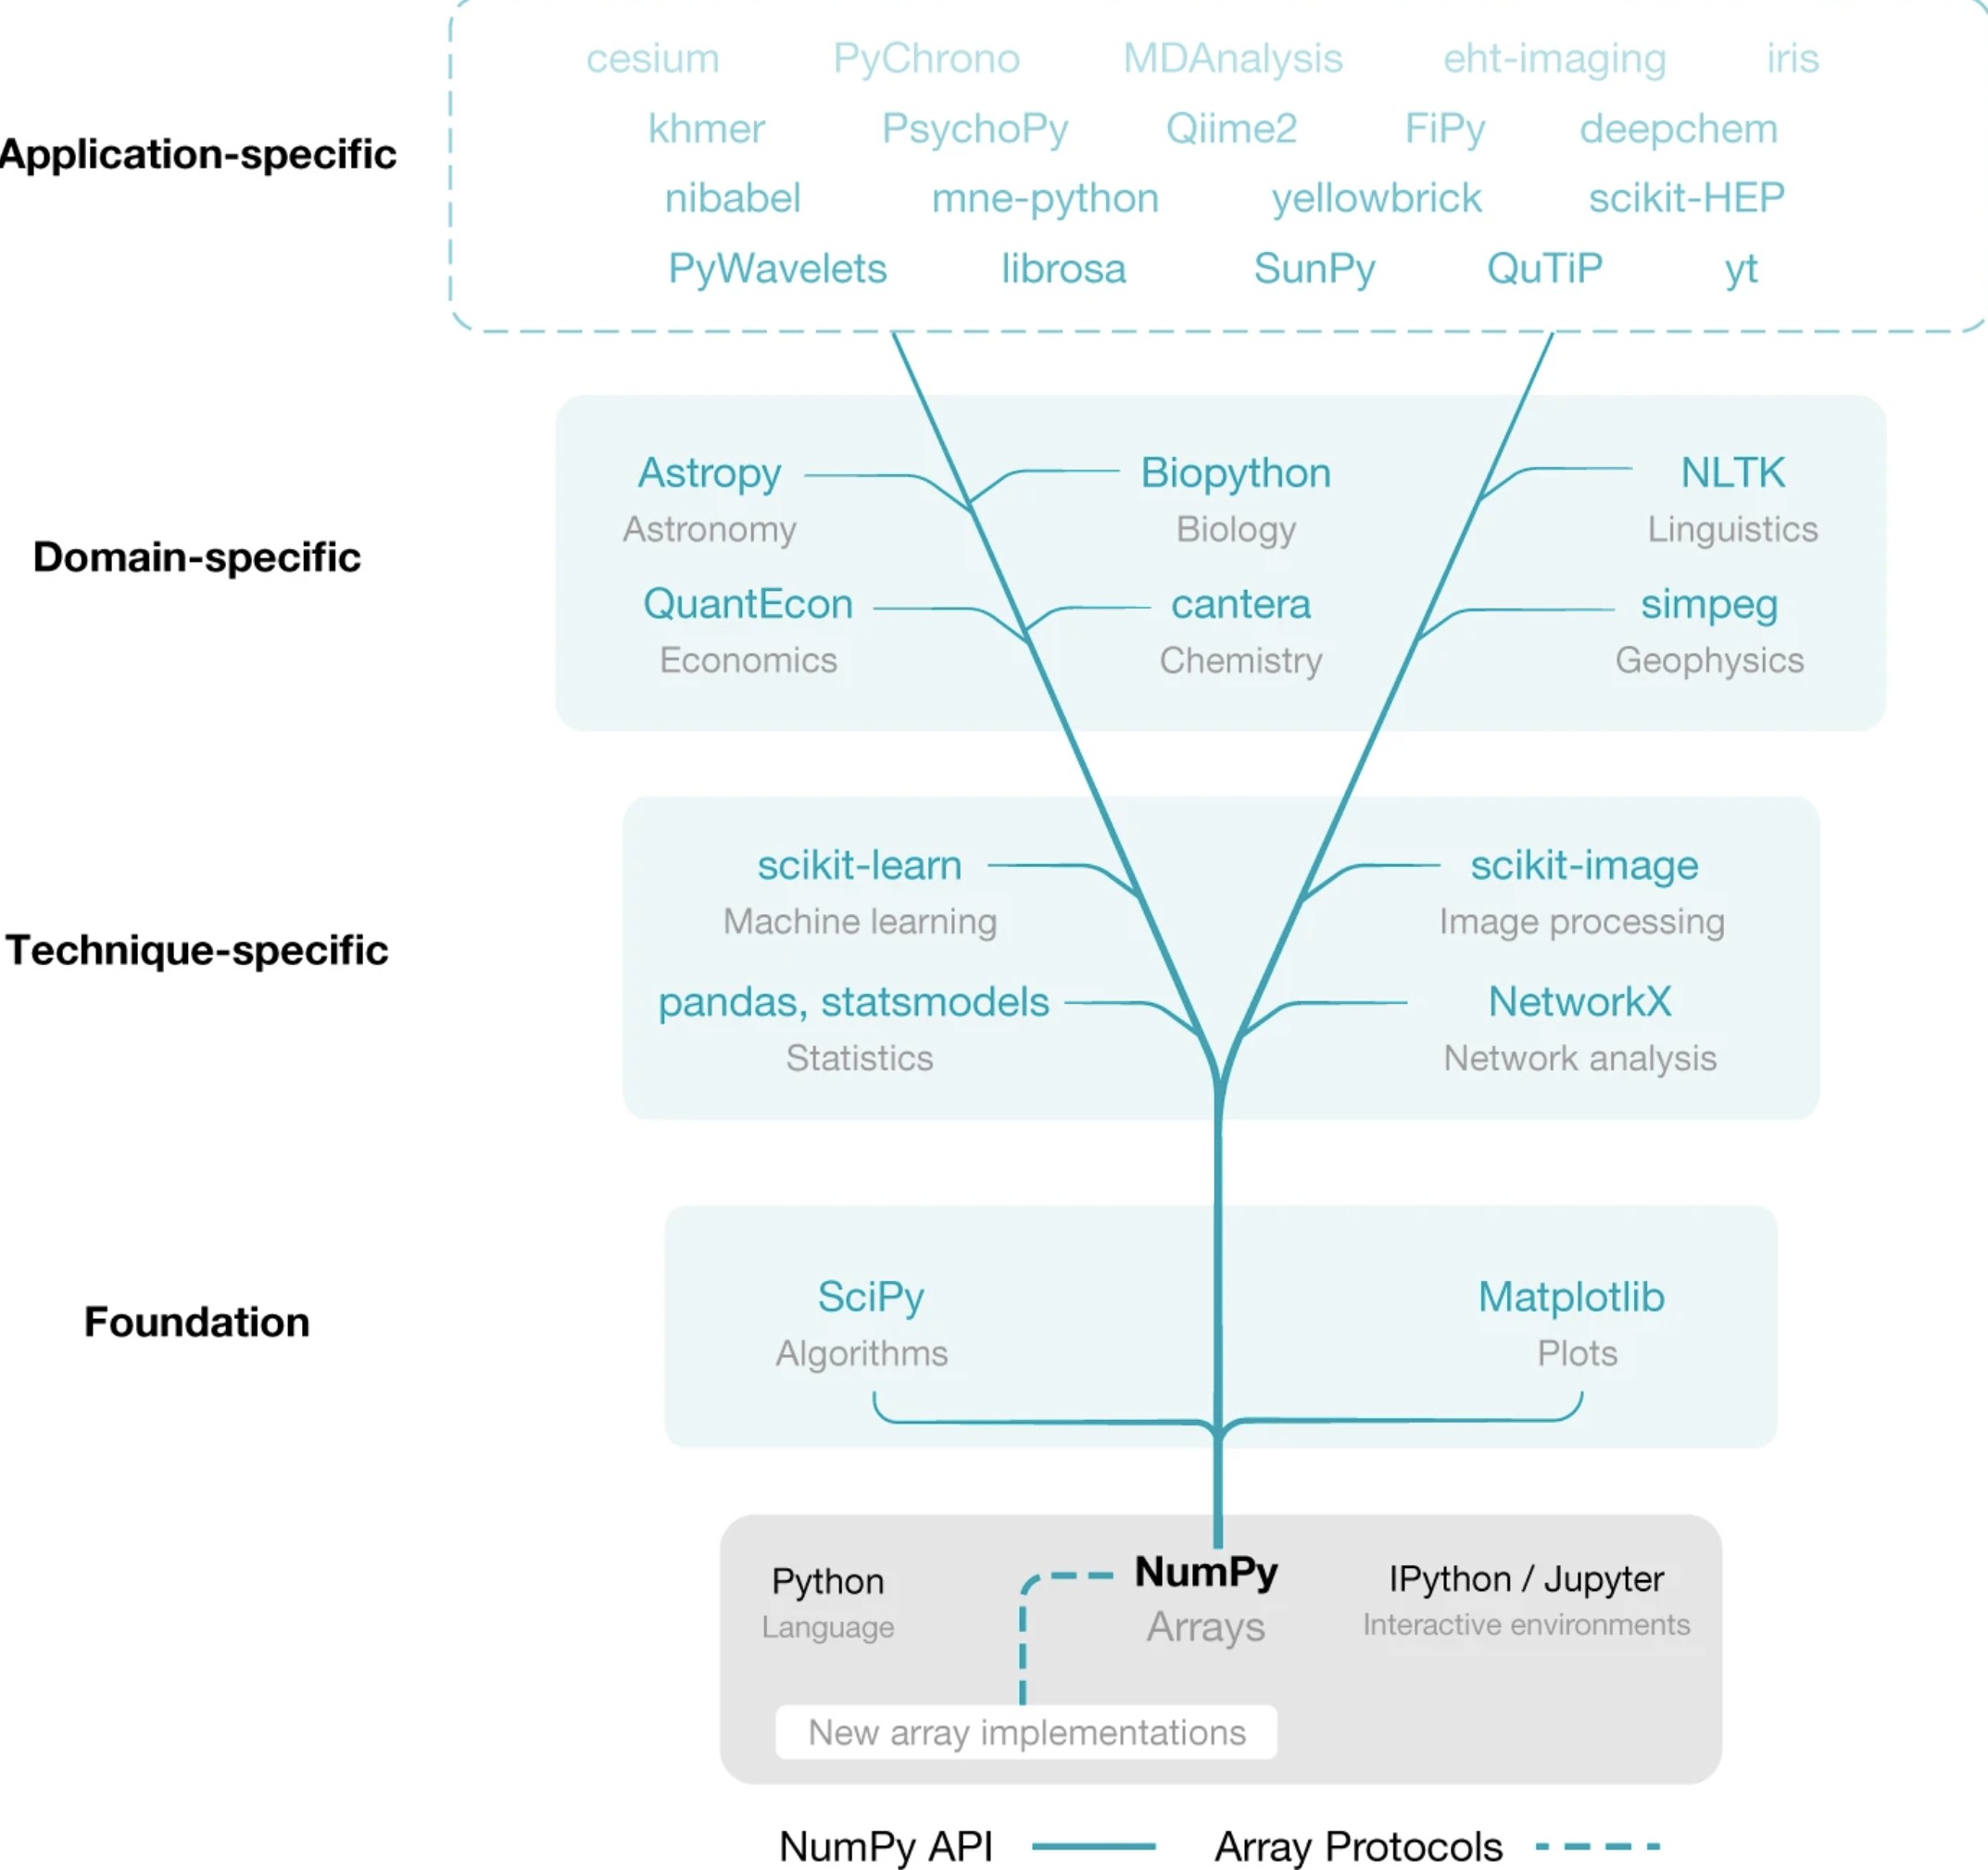
\includegraphics[width=\textwidth]{numpy_related_packs.png}}
\caption{گراف وابستگی کتاب‌خانه‌های پایتون به \lr{NumPy}\cite{van2011numpy}}
\label{fig:numpy_related_packs}
\end{figure}

\subsection{کتاب‌خانه‌ی \lr{Scikit-Learn}} 
\lr{Scikit-Learn}، جامع‌ترین و بزرگ‌ترین بسته یادگیری ماشین منبع‌باز در پایتون است. چون یادگیری ماشین اغلب بعنوان یک جزء از یک برنامه عمومی‌تر (همانند پروژه‌ی کنونی که به عنوان یک سرویس در وب توسعه داده‌شده است) استفاده می‌شود، ایده‌آل است که از همان زبان برنامه‌نویسی استفاده شود تا بصورت یکپارچه با سایر بخش‌های برنامه هماهنگ شود. با استفاده از قابلیت‌های گسترده پایتون، \lr{Scikit-Learn} بعنوان یک بسته محبوب برای برنامه‌های مرتبط با یادگیری ماشین در حال رشد است\cite{hao2019machine}. این کتاب‌خانه شامل توابع و اشیاء فراوانی برای مسائل طبقه‌بندی، رگرسیون، تقریب ماتریس کوواریانس، کاهش بعد و پیش‌پردازش داده‌ی خام می‌باشد\cite{kramer2016scikit}. اگرچه پایتون یک زبان برنامه‌نویسی تفسیری است، اما بیشتر روش‌های یادگیری ماشین در \lr{Scikit-Learn} بر پایه کتابخانه‌های دودویی کامپایل شده است که در ابتدا با زبان‌های فورتران\LTRfootnote{Fortran}، سی یا سی‌پلاس‌پلاس\LTRfootnote{C++} برنامه‌نویسی شده‌اند. این پیاده‌سازی‌های مبتنی بر دودویی‌ها بطور قابل‌توجهی کارایی محاسبات را بهبود می‌بخشند\cite{hao2019machine, kramer2016scikit}.

\subsection{کتاب‌خانه‌‌های جانبی}
در این پروژه برای توسعه‌ی بدون خطای سرویس‌های مختلف، از کتاب‌خانه‌های جانبی دیگری نیز استفاده‌شده است که در اینجا به آنها و موارد کاربردشان اشاره می‌کنیم.
\begin{itemize}

\item \textbf{\lr{PyJWT} و \lr{Werkzeug}}: از این دو کتاب‌خانه برای توسعه‌ی سرویس احراز هویت مدیران و دروازه‌های ارسال‌کننده‌ی داده‌های مربوط به لرزش با کمک استاندارد \lr{JWT} استفاده کرده‌ایم.

\item \textbf{\lr{Pandas}}: برای کارهایی همانند خواندن مجموعه‌ی داده\LTRfootnote{Dataset} و پردازش روی آنها از این کتاب‌خانه کمک گرفته شد.

\item \textbf{\lr{SQLAlchemy}}: این کتاب‌خانه بدلیل در اختیار گذاشتن رابط‌های برنامه‌نویسی\LTRfootnote{Application Programming Interface (API)} مناسب برای ارتباط با پایگاه‌داده‌های رابطه‌ای، بسیار محبوب است و در این پروژه نیز از آن استفاده کرده‌ایم.

\end{itemize}


\section{پایگاه داده‌ی رابطه‌ای}
پایگاه داده برنامه‌ای برای ذخیره و بازیابی سریع حجم فراوانی از داده و بصورت مکرر می‌باشد. پایگاه داده‌ی رابطه‌ای\LTRfootnote{Relational Database} در سال ۱۹۷۰ میلادی معرفی شد. داده در این نوع از پایگاه داده بشکل جداولی\LTRfootnote{Tables} (از جدول به عنوان رابطه\LTRfootnote{Relation} نیز یاد می‌شود) ذخیره می‌شود و می‌تواند به شکل‌های متفاوت به آن دسترسی پیدا کرد یا آن را تغییر داد. هر ستون این جدول نشان‌دهنده‌ی یک مشخصه و هر سطر نماینده‌ی یک موجودیّت از آن رابطه می‌باشد. هر کدام از این جداول می‌توانند با همدیگر ارتباط داشته‌ باشند. از این‌رو به این نوع از پایگاه داده، پایگاه داده‌ی رابطه‌ای گفته می‌شود\cite{jatana2012survey}. از معروف‌ترین پایگاه‌داده‌های رابطه‌ای می‌توان به \lr{MySQL}، \lr{PostgreSQL}، \lr{Oracle Database} و \lr{Microsoft SQL Server} اشاره کرد.

اکثر پایگاه‌های داده رابطه‌ای از زبان پرسمان ساختاریافته\LTRfootnote{Structured Query Language (SQL)} برای دسترسی و اصلاح داده‌های ذخیره شده در پایگاه داده استفاده می‌کنند. برای انجام این پروژه از \href{https://www.postgresql.org/}{\lr{PostgreSQL}} که یکی معروف‌ترین پایگاه‌ داده‌ی رابطه‌ای متن‌باز است، استفاده کرده‌ایم(لوگوی آن در \cref{fig:postgres_logo}\cite{postgresqlPostgreSQL} آورده شده است).

\begin{figure}[!h]
\centerline{
\includegraphics[width=0.2\textwidth]{postgres_logo.png}}
\caption{لوگوی \lr{PostgreSQL}، یکی از معروف‌ترین پایگاه داده‌های رابطه‌ای\cite{postgresqlPostgreSQL}}
\label{fig:postgres_logo}
\end{figure}

\section{داکر}
داکر\LTRfootnote{Docker} در حال حاضر معروف‌ترین و پراستفاده‌ترین ابزار برای پیاده‌سازی معماری سرویس‌های کوچک\LTRfootnote{Microservices} و استقرار آنها روی ابر است.  وظیفه‌ی اصلی و واحد داکر این است که با بسته‌بندی برنامه‌ها و متعلقات آن بصورت واحدی به نام کانتینر\LTRfootnote{Container}، امکان استفاده و کار کردن آنها را روی هر ماشینی که موتور داکر روی آن نصب شده است را تضمین کند. هر یک از کانتینرهای داکر در یک محیط مجزا و با منابع متفاوت تخصیص داده‌شده توسط موتور داکر، اجرا می‌شوند. این مدل اجرای ایزوله‌ی کانتینرهای داکر سبب قابل حمل‌بودن واحدهای مختلف اجرایی برنامه، مقیاس‌پذیری راحت برنامه‌های مختلف و همچنین انعطاف‌پذیری بالا نسبت به محیط اجرایی و شرایط وابسته به آن خواهد شد\cite{anderson2015docker, dockerDockerOverview}.

سرویس داکر همانطور که در \cref{fig:docker_architecture}\cite{dockerDockerOverview} مشخص است، خود از چندین بخش مجزا تشکیل‌شده است که در این قسمت آنها را شرح 
خواهیم داد. داکر از معماری مشتری-کارگزار\LTRfootnote{Client-Server} استفاده می کند. در ساختار داکر، \lr{Docker Client} با \lr{Docker Daemon} که کارهایی همانند ساخت، اجرا و توزیع کانتینرهای داکری را انجام می دهد، صحبت می‌کند. سرویس‌های \lr{Docker Client} و \lr{Docker Daemon} می‌توانند روی یک سیستم اجرا شوند، یا می‌توانند روی دو ماشین متفاوت باشند و با یکدیگر ارتباط برقرار کنند. این دو سرویس با استفاده از رابط کاربری برنامه‌نویسی، با همدیگر تعامل می‌کنند. یکی دیگر از سرویس‌گیرندگان معروف داکر، \lr{Docker Compose} است که امکان ایجاد و اجرای چند کانتینر داکری را بصورت همزمان برقرار می‌کند. همانطور که فهمیدیم، واحد‌های اجرایی در داکر، کانتینر نامیده می‌شوند. نکته‌ی قابل‌توجه در اینجا این است که این واحد‌های اجرایی از واحد‌هایی به‌نام ایمیج ساخته و اجرا می‌شوند. هنگامی که \lr{Docker Daemon} درخواست جدیدی برای بالا آوردن یک کانتینر از \lr{Docker Client} دریافت می‌کند، در صورتی که ایمیج داکری روی سیستم میزبان قرار داشت بلافاصله شروع به تخصیص منابع و شروع کانتینر مربوطه می‌کند. در غیر این صورت، از واحدی به‌نام \lr{Docker Registry} ایمیج مربوطه را دریافت و سپس همان روند قبلی را طی می‌کند \cite{dockerDockerOverview}.

\begin{figure}[!h]
\centerline{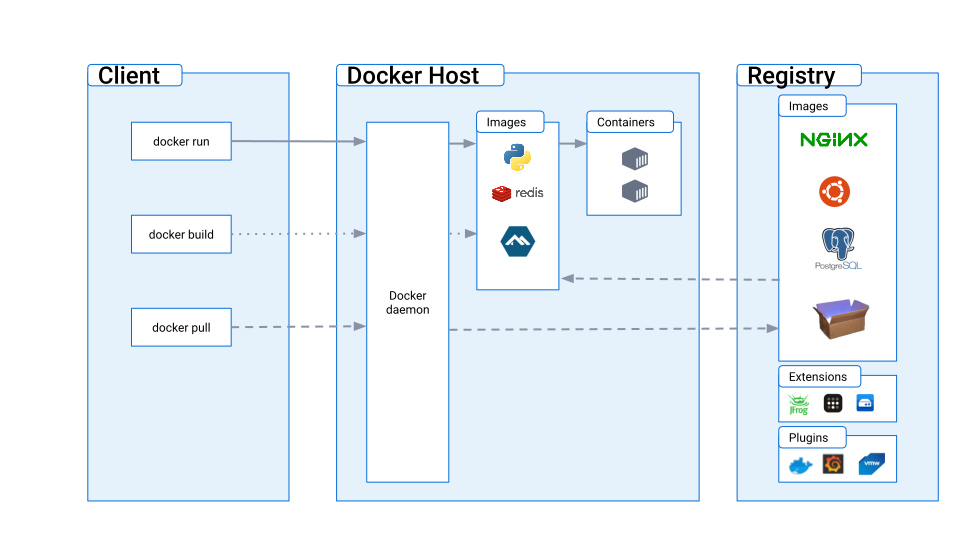
\includegraphics[width=\textwidth]{docker_architecture.png}}
\caption{معماری داکر\cite{dockerDockerOverview}}
\label{fig:docker_architecture}
\end{figure}

توسعه‌ی داکر در واقع تلاشی برای رفع مشکلات استفاده از ماشین‌های مجازی\LTRfootnote{Virtual Machines} بود. کانتینرهای داکر و ماشین‌های مجازی مطابق \cref{fig:docker_vs_vm} در نحوه‌ی مجازی‌سازی و استفاده از منابع کامپیوتر با یکدیگر متفاوت‌اند. ماشین‌های مجازی منابع سخت‌افزاری سیستم را بین خود تقسیم می‌کنند و بدلیل وجود لایه‌ای اضافی برای ایجاد دستورات قابل‌فهم برای لایه‌ی سخت‌افزار، نسبت به کانتینرهای داکر که منابع سیستم‌عامل را بین خود تقسیم می‌کنند و یک لایه کمتر دارند، کندتر اجرا می‌شوند و سربار بشدت بالاتری را متحمل می‌شوند\cite{anderson2015docker, yadav2019docker}.

\begin{figure}[!h]
\centerline{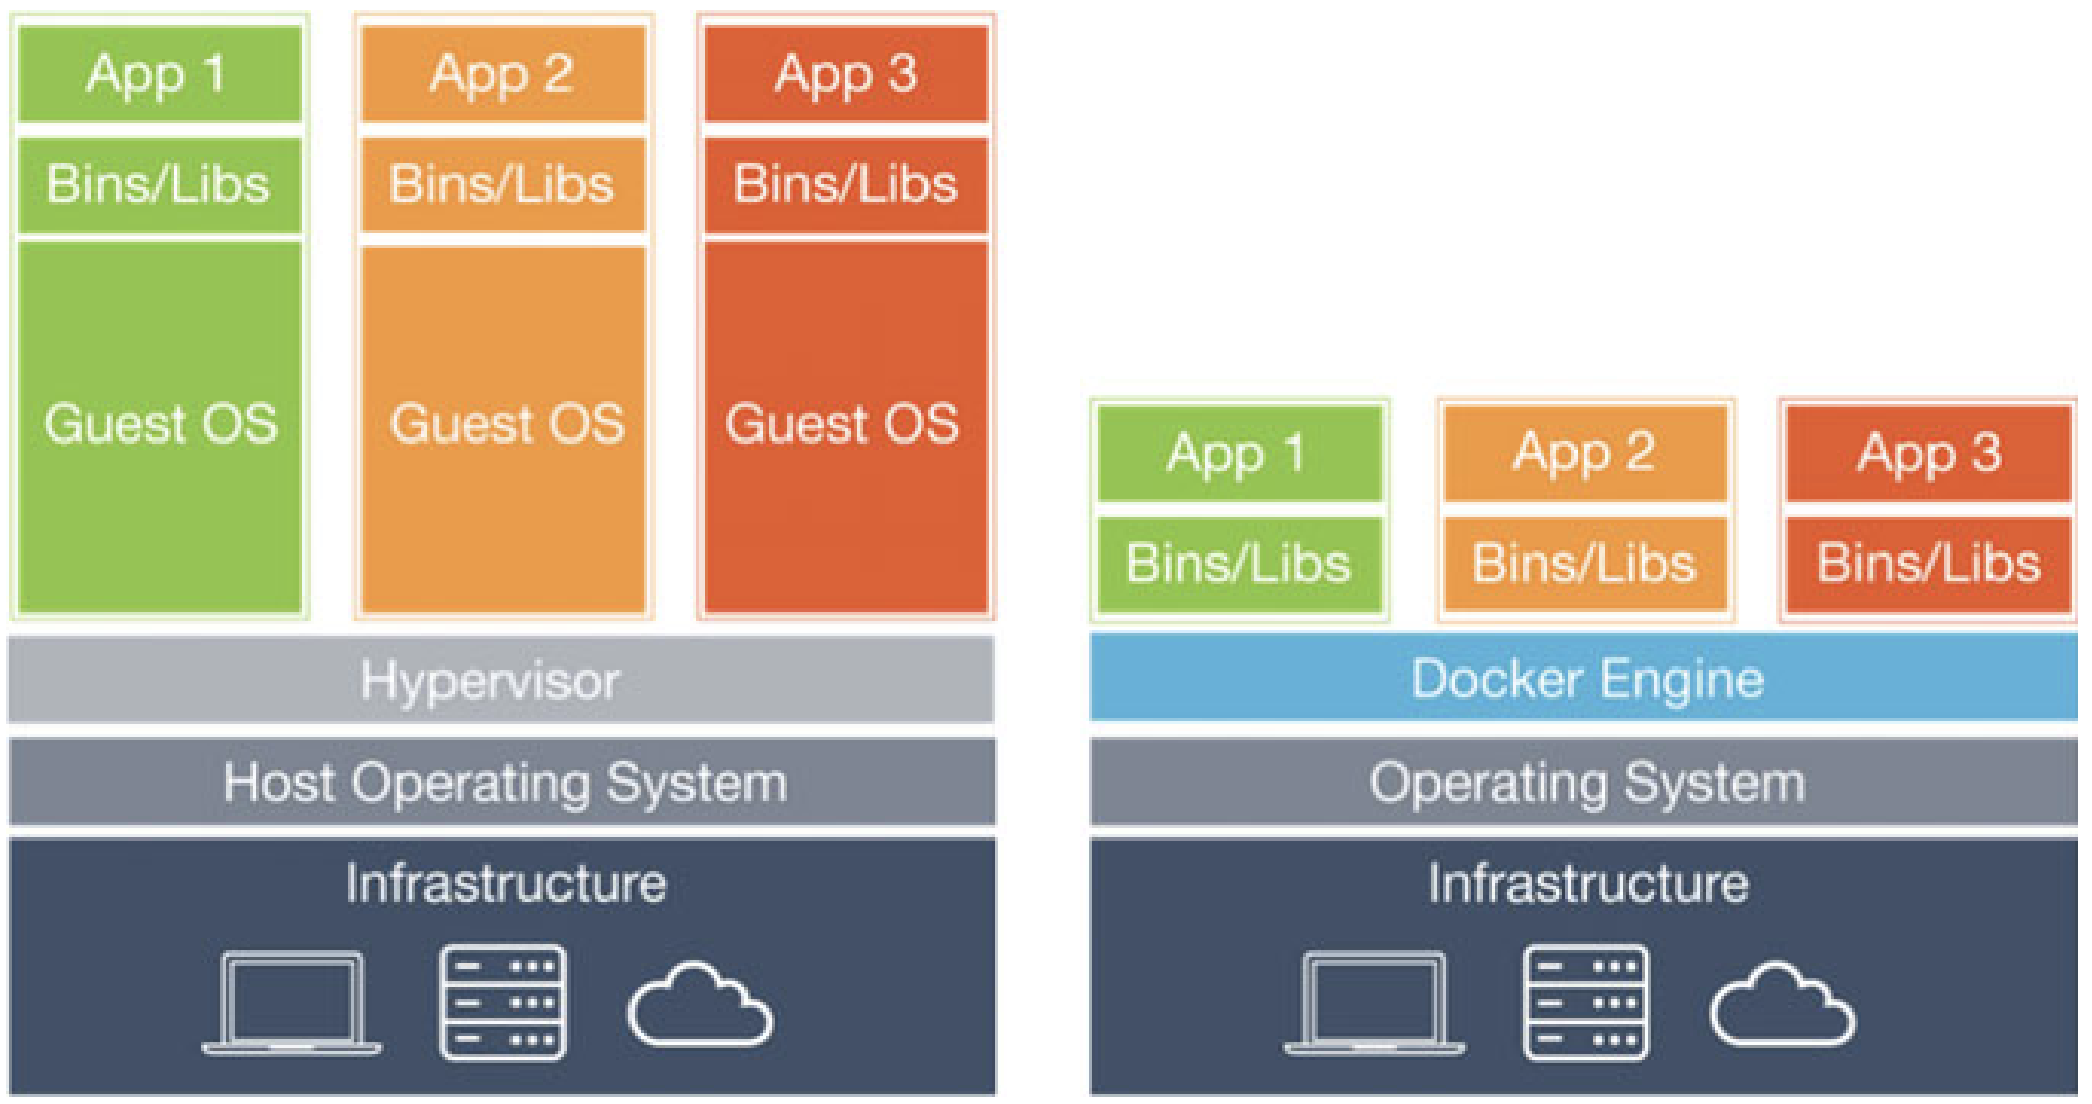
\includegraphics[width=\textwidth]{docker_vs_vm.png}}
\caption{ماشین‌های مجازی در برابر کانتینرهای داکری\cite{yadav2019docker}}
\label{fig:docker_vs_vm}
\end{figure}

\section{جمع‌بندی و نتیجه‌گیری}
در این بخش، به تکنولوژی‌ها و چارچوب‌های اصلی استفاده‌شده برای توسعه‌ی مدل یادگیری ماشین اشاره کردیم. همانطور که در طول فصل بدان اشاره شد، زبان پایتون بدلیل دارابودن غنی‌ترین کتابخانه‌های مربوط به محاسبات و یادگیری ماشین منطقی‌ترین انتخاب ممکن برای برگزیدن زبان توسعه‌ی مدل و سرویس هوش‌مصنوعی بود. دارابودن چارچوب‌های با کارایی بالا برای توسعه برنامه‌ی وب نیز دیگر دلیل مهم برای انتخاب پایتون است. در مرحله‌ی بعد پایگاه‌های داده‌ی رابطه‌ای را معرفی کردیم و تا حدودی با نحوه‌ی ذخیره‌ و بازیابی داده در آنها آشنا شدیم و مشخص کردیم که از پایگاه داده‌ی \lr{PostgreSQL} که یک پایگاه‌ داده‌ی رابطه‌ای متن‌باز است، برای انجام این پروژه بهره‌ بردیم. در انتهای این بخش نیز ابزار داکر را معرفی کردیم و اجزا و قسمت‌های متفاوت آن را بررسی کردیم و همچنین مزایای آن نسبت به ماشین‌های مجازی که روش سنتی استقرار برنامه‌ها روی ابر بود را بر شمردیم.  